\begin{*anmerkung}
	Der Inhalt dieses ganzen Kapitels ist eigentlich nicht prüfungsrelevant.
\end{*anmerkung}

\section{Addition $n$-stelliger ganzer Zahlen}

Wir werden im Folgenden folgende Notationen verwenden:
\begin{itemize}
	\item OR: $x+y$
	\item AND: $x\cdot y$
	\item NOT: $\overline{x}$
	\item XOR: $x\oplus y$
\end{itemize}

Beim \begriff{Halbaddierer} ist die Summe $s=a\oplus b$ und der Übertrag (carry) $c=a\cdot b$.

\begin{figure}[ht]
	\centering
	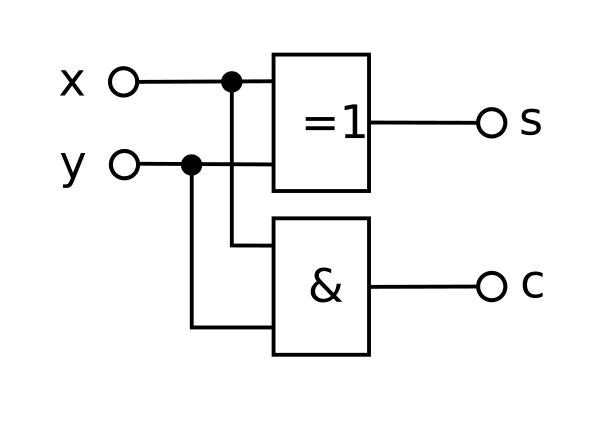
\includegraphics{images/Halbaddierer.png}
	\caption{Halbaddierer}
\end{figure}

Der \begriff{Volladdierer} besteht aus 2 Halbaddierern. Die Summe $s$ ist hier: $s=a\overline{b}\overline{c_{in}}+\overline{a}b\overline{c_{in}}+\overline{a}\overline{b}c_{in}+abc_{in}+a\oplus b\oplus c_{in}$. Der Übertrag ist $c_{out}=ab+ac_{in}+bc_{in}$.

\begin{figure}[ht]
	\centering
	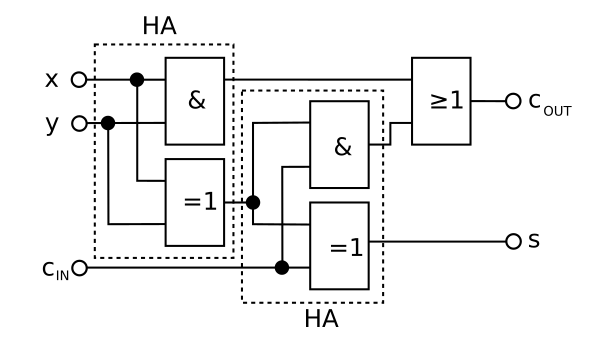
\includegraphics{images/Volladdierer.png}
	\caption{Volladdierer}
\end{figure}

Mit dem \begriff{Carry-Ripple-Adder} kann man dann endlich zwei $n$-stellige Zahlen addieren:
\begin{itemize}
	\item $a=[a_{n-1}a_{n-2}...a_1a_0]_2$
	\item $b=[b_{n-1}b_{n-2}...b_1b_0]_2$
\end{itemize}

\begin{figure}[ht]
	\centering
	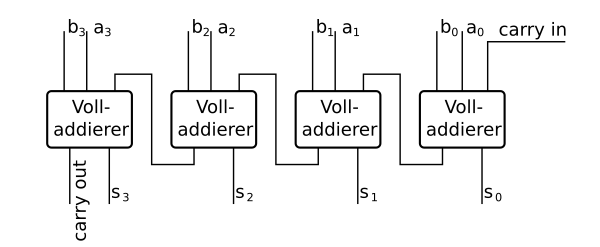
\includegraphics{images/Carry-Ripple-Adder.png}
	\caption{Carry-Ripple-Adder}
\end{figure}
$\Rightarrow T(n)=\mathcal{O}(n\cdot T_{FA})$

Machen wir zum Schluss noch eine Übertragsanalyse: Eine Bitposition $i\in\{0,1,...,n-1\}$ kann 3 verschiedene Übertragsfälle annehmen:
\begin{enumerate}
	\item kein Übertrag möglich, wenn $a_i=b_i=0$
	\item Übertrag wird weitergeleitet (\begriff{carry propergate}) $p=a_i\oplus b_i$
	\item Übertrag wird auf jeden Fall generiert (\begriff{generate bit}) $g=a_i\cdot b_i$
\end{enumerate}

Rekursionsbeziehung:
\begin{align}
	c_{i+1} &= g_i+p_i\cdot c_i=a_ib_i+(a_i\oplus b_i)c_i=a_ib_i+(a_i+b_i)c_i \notag \\
	c_{i+1} &= \underbrace{g_i+p_ig_{i-1}+p_ip_{i-1}g_{i-2}+...+p_ip_{i-1}...p_1g_0}_{G_{0,i}} + \underbrace{p_ip_{i-1}...p_1p_0}_{P_{0,i}}\cdot c_0\notag
\end{align}